\section{Lezione 10}
\subsection{Ripasso e approfondimento: teoria dell'integrazione secondo Riemann}
\begin{definition}
    \label{def:8.1}
    Sia $f\colon[a,b]\to\amsbb{R}$ una funzione \textbf{limitata definita su} $\mathbf{[a,b]}$. Una \emph{partizione} $\mathscr{P}$ di $[a,b]$ è una collezione di punti $\{x_0, \dots, x_n\}\subset [a,b]$ tale che
    \[
    a=x_0 < x_1 < \dots < x_{n-1}<x_n= b
    \]
    Data una partizione $\mathscr{P}$ di $[a,b]$ e la funzione $f$, definiamo le quantità
    \begin{equation}
        \label{eq:8.1}
        \Delta_i = x_i - x_{i-1} \qquad M_i = \sup_{x\in[x_i, x_{i-1}]} f(x) \qquad m_i = \inf_{x\in[x_i, x_{i-1}]} f(x)
    \end{equation}
    con cui definiamo la somma di Darboux superiore $U(\mathscr{P}, f)$ e inferiore $L(\mathscr{P},f)$
    \[
    \underbrace{U(\mathscr{P},f) = \sum_{i=1}^n M_i \Delta_i}_{\stepcounter{equation}\mbox{(\theequation)}} \qquad \underbrace{L(\mathscr{P},f) = \sum_{i=1}^n m_i \Delta_i}_{\stepcounter{equation}\mbox{(\theequation)}}
    \]
    \addtocounter{equation}{-2}\refstepcounter{equation}\label{eq:8.2}
    \addtocounter{equation}{0}\refstepcounter{equation}\label{eq:8.3}
\end{definition}
\begin{remark}
    Notiamo che somma superiore ed inferiore ammettono un'interessante interpretazione grafica. Nei grafici successivi riportiamo, data una generica funzione $f$ e una partizione $\mathscr{P}= \{x_0, \dots, x_6\}$ di $[a,b]$, la somma superiore $U(\mathscr{P},f)$ e inferiore $L(\mathscr{P},f)$:  
    \begin{center}
    \begin{minipage}{.45\linewidth}
        \centering
        \begin{tikzpicture}[scale=1.4, font=\footnotesize]
            \tzaxes(-1.2,-0.5)(3.3,2.7){$x$}[b]
            \tzticks{-.5/$a$, 0.6/$x_2$, 1.4/$x_4$, 2.6/$b$}[b]
            \tzticks*{-.5/$a$, 0.2/$x_1$, 0.6/$x_2$, 1.2/$x_3$, 1.4/$x_4$, 2.1/$x_5$, 2.6/$b$}
            \tzticks{0.2/$x_1$, 1.2/$x_3$, 2.1/$x_5$}[a]
            \tzfn[black]"curve"{cos(3*deg(\x))+sin(.9*deg(\x))+0.5}[-.5:2.6]{$f(x)$}[br]
            \tzpolygon*[blue,auto,dashed,text=black]
             (-0.5,0)(0.2,0)(0.2,1.5452)(-0.5,1.5452);
            \tzpolygon*[blue,auto,dashed,text=black]
             (0.2,0)(0.6,0)(0.6,1.5043)(0.2,1.5043);
            \tzpolygon*[blue,auto,dashed,text=black]
             (0.6,0)(1.2,0)(1.2,0.7869)(0.6,0.7869);
            \tzpolygon*[blue,auto,dashed,text=black]
             (1.2,0)(1.4,0)(1.4,0.9618)(1.2,0.9618);
            \tzpolygon*[blue,auto,dashed,text=black]
             (1.4,0)(2.1,0)(2.1,2.455)(1.4,2.455);
            \tzpolygon*[blue,auto,dashed,text=black]
             (2.1,0)(2.6,0)(2.6,2.4493)(2.1,2.4493);
        \end{tikzpicture}
    \end{minipage}
    \hspace{1pt}
    \begin{minipage}{.45\linewidth}
        \centering
        \begin{tikzpicture}[scale=1.4, font=\footnotesize]
            \tzaxes(-1.2,-0.5)(3.3,2.7){$x$}[b]
            \tzticks{-.5/$a$, 0.6/$x_2$, 1.4/$x_4$, 2.6/$b$}[b]
            \tzticks*{-.5/$a$, 0.2/$x_1$, 0.6/$x_2$, 1.2/$x_3$, 1.4/$x_4$, 2.1/$x_5$, 2.6/$b$}
            \tzticks{0.2/$x_1$, 1.2/$x_3$, 2.1/$x_5$}[a]
            \tzfn[black]"curve"{cos(3*deg(\x))+sin(.9*deg(\x))+0.5}[-.5:2.6]{$f(x)$}[br]
            \tzpolygon*[red,auto,dashed,text=black]
             (-0.5,0)(0.2,0)(0.2,0.1358)(-0.5,0.1358);
            \tzpolygon*[red,auto,dashed,text=black]
             (0.2,0)(0.6,0)(0.6,0.7869)(0.2,0.7869);
            \tzpolygon*[red,auto,dashed,text=black]
             (0.6,0)(1.2,0)(1.2,0.2922)(0.6,0.2922);
            \tzpolygon*[red,auto,dashed,text=black]
             (1.2,0)(1.4,0)(1.4,0.4852)(1.2,0.4852);
            \tzpolygon*[red,auto,dashed,text=black]
             (1.4,0)(2.1,0)(2.1,0.9618)(1.4,0.9618);
            \tzpolygon*[red,auto,dashed,text=black]
             (2.1,0)(2.6,0)(2.6,1.2724)(2.1,1.2724);
        \end{tikzpicture}
    \end{minipage}
\end{center}
Come si può osservare, $U(\mathscr{P}, f)$ approssima l'area sottesa dal grafico di $f$ dall'alto, mentre $L(\mathscr{P}, f)$ la approssima dal basso. Notiamo inoltre come queste due quantità dipendano sia dalla funzione $f$ considerata, sia dalla scelta della partizione $\mathscr{P}$, e che
\begin{equation}
    \label{eq:8.4}
    \left(\sup_{x\in[a,b]}f(x)\right)(b-a)\ge U(\mathscr{P}, f) \ge L(\mathscr{P},f) \ge \left(\inf_{x\in[a,b]}f(x)\right)(b-a) \ \text{per ogni} \ \mathscr{P}
\end{equation}
\end{remark}
\begin{definition}
    \label{def:8.2}
    Chiamiamo \emph{integrale inferiore} di $f$ su $[a,b]$ la quantità
    \[
    \bint_a^b f = \sup_{\mathscr{P}} L(\mathscr{P},f)
    \]
    ossia l'estremo superiore, preso su tutte le possibili partizioni $\mathscr{P}$ di $[a,b]$, dell'insieme delle somme inferiori. Analogamente, chiamiamo \emph{integrale superiore} di $f$ su $[a,b]$ la quantità
    \[
    \aint_a^b f = \inf_{\mathscr{P}} U(\mathscr{P},f)
    \]
    ossia l'estremo inferiore, preso su tutte le possibili partizioni $\mathscr{P}$ di $[a,b]$, dell'insieme delle somme superiori. Notiamo che queste due quantità sono sempre ben definite per una funzione limitata, in quanto vale la (\ref{eq:8.4}) (e ci ricordiamo il teorema \ref{th:2.1} e il corollario \ref{cor:2.1}). Diremo che $f$ è \emph{Riemann-integrabile} su $[a,b]$ ($f\in\mathscr{R}([a,b])$) se
    \[
    \bint_a^b f = \aint_a^b f
    \]
    è in tal caso il valore comune verrà denotato con
    \[
    \int_a^b f = \int_a^b f(x)\, dx 
    \]
    e verrà detto \emph{integrale di $f$ su $[a,b]$}.
\end{definition}
\begin{remark}
    Notiamo che in generale vale che
    \[
    \bint_a^b f \le \aint_a^b f
    \]
    Per mostrare la validità della disuguaglianza, procediamo come di seguito:
    \begin{enumerate}[(i)]
        \item Data una partizione $\mathscr{P}$ di $[a,b]$, un suo \emph{raffinamento} $\mathscr{Q}$ è una partizione tale che $\mathscr{P}\subseteq \mathscr{Q}$. Date due partizioni $\mathscr{P}_1$ e $\mathscr{P}_2$, il loro raffinamento comune sarà dato da $\mathscr{P}_1 \cup \mathscr{P}_2$.
        \item Se $\mathscr{Q}$ è un raffinamento di $\mathscr{P}$, allora vale che
        \[
        L(\mathscr{P}, f) \le L(\mathscr{Q},f) \qquad U(\mathscr{Q},f)\le U(\mathscr{P},f)
        \]
        Per mostrare che valgono queste due disuguaglianze, consideriamo il caso base in cui $\mathscr{Q} = \mathscr{P} \cup \{\overline{x}\}$, $x_{i-1} < \overline{x}<x_i$ per qualche $i$. Definiamo
        \[
        \overline{m}_1 = \inf_{x\in[x_{i-1}, \overline{x}]}f(x) \qquad \overline{m}_2 = \inf_{x\in[\overline{x}, x_i]}f(x)
        \]
        e notiamo che
        \[
        \overline{m}_1 \ge m_i \qquad \overline{m}_2 \ge m_i
        \]
        A questo punto vale che
        \[
        \begin{split}
            L(\mathscr{Q}, f)-L(\mathscr{P},f) &= \sum_{k=1}^{i-1}m_k \Delta_k + \overline{m}_1 (\overline{x}-x_{i-1}) + \overline{m}_2 (x_i - \overline{x}) + \sum_{k=i+1}^n m_k \Delta_k - \\
            & -\sum_{k=1}^n m_k \Delta_k = \overline{m}_1 (\overline{x}-x_{i-1}) + \overline{m}_2 (x_i - \overline{x})-m_i(x_{i}-x_{i-1})\ge \\
            & \ge m_i(\overline{x}-x_{i-1}) + m_i (x_i -\overline{x})-m_i(x_i-x_{i-1}) = 0
        \end{split}
        \]
        Il risultato si dimostra analogamente per $U(\mathscr{Q}, f) \le U(\mathscr{P},f)$.
        \item Per il punto precedente vale che, date due generiche partizioni $\mathscr{P}_1$ e $\mathscr{P}_2$ e indicando con $\mathscr{Q}$ il loro raffinamento comune,
        \[
        L(\mathscr{P}_1, f)\le L(\mathscr{Q}, f) \le U(\mathscr{Q}, f)\le U(\mathscr{P}_2, f)
        \]
        ossia
       \begin{equation}
           \label{eq:8.5}
           L(\mathscr{P}_1, f)\le U(\mathscr{P}_2, f) \ \text{per ogni} \ \mathscr{P}_1, \mathscr{P}_2
       \end{equation}
       Fissiamo a questo punto $\mathscr{P}_1$; vale che
       \[
       L(\mathscr{P}_1, f)\le U(\mathscr{P}_2, f) \ \forall \mathscr{P}_2 \implies L(\mathscr{P}_1, f)\le \aint_a^b f
       \]
       Poiché la partizione $\mathscr{P}_1$ che avevamo fissato era generica, allo stesso modo vale che
       \[
       L(\mathscr{P}_1, f)\le \aint_a^b f \ \forall \mathscr{P}_1 \implies \bint_a^b f \le \aint_a^b f
       \]
    \end{enumerate}
\end{remark}
\begin{theorem}[Criterio di Riemann]
    \label{th:8.1}
    Una funzione $f\colon [a,b]\to \amsbb{R}$ limitata su $[a,b]$ è Riemann-integrabile se e solo se per ogni $\varepsilon>0$ esiste una partizione $\mathscr{P}_\varepsilon$ di $[a,b]$ tale che
    \[
    U(\mathscr{P}_\varepsilon, f) - L(\mathscr{P}_\varepsilon, f)< \varepsilon
    \]
\end{theorem}
\begin{proof}
    Mostriamo le due implicazioni.
    \begin{enumerate}[(i)]
        \item Supponiamo che $f\in\mathscr{R}([a,b])$. Notiamo che per ogni partizione $\mathscr{P}$ di $[a,b]$ vale che
        \[
        L(\mathscr{P},f) \le \bint_a^b f \le \aint_a^b f \le U(\mathscr{P}, f)
        \]
        Per definizione (cfr. definizione \ref{def:2.2}) di estremo superiore, per ogni $\varepsilon>0$ esiste una partizione $\mathscr{P}_1$ tale che
        \[
        L(\mathscr{P}_1, f) > \bint_a^b f -\frac{\varepsilon}{2} \iff L(\mathscr{P}_1, f) + \frac{\varepsilon}{2}> \bint_a^b f
        \]
        e allo stesso modo per definizione di estremo inferiore per ogni $\varepsilon>0$ esiste una partizione $\mathscr{P}_2$ tale che
        \[
        U(\mathscr{P}_2, f) < \aint_a^b f +\frac{\varepsilon}{2} \iff U(\mathscr{P}_2, f) - \frac{\varepsilon}{2}<\aint_a^b f
        \]
        Definiamo $\mathscr{P}_\varepsilon = \mathscr{P}_1\cup \mathscr{P}_2$; vale che
        \[
        U(\mathscr{P}_\varepsilon, f) \le U(\mathscr{P}_2, f) < \underbrace{\bint_a^bf +\frac{\varepsilon}{2} = \aint_a^b f -\frac{\varepsilon}{2}+\varepsilon}_{\text{Definizione \ref{def:8.2}}} < L(\mathscr{P}_1, f)+\varepsilon \le L(\mathscr{P}_\varepsilon, f) + \varepsilon
        \]
        ossia abbiamo trovato, per ogni $\varepsilon>0$, una partizione $\mathscr{P}_\varepsilon$ tale che
        \[
        U(\mathscr{P}_\varepsilon, f) < L(\mathscr{P}_\varepsilon, f) + \varepsilon \iff U(\mathscr{P}_\varepsilon, f) - L(\mathscr{P}_\varepsilon, f) <  \varepsilon
        \]
        \item Supponiamo che per ogni $\varepsilon>0$ esista una partizione $\mathscr{P}_\varepsilon$ tale che
        \[
        U(\mathscr{P}_\varepsilon, f) - L(\mathscr{P}_\varepsilon, f)< \varepsilon
        \]
        Sappiamo che $U(\mathscr{P}_\varepsilon, f)\ge \aint_a^b f$ e che $L(\mathscr{P}_\varepsilon, f)\le \bint_a^b f$; quindi
        \[
        \varepsilon>U(\mathscr{P}_\varepsilon, f) - L(\mathscr{P}_\varepsilon, f) \ge \aint_a^b f - L(\mathscr{P}_\varepsilon, f) \ge \underbrace{\aint_a^b f - \bint_a^b f\ge 0}_{\text{Osservazione precedente}}
        \]
        ossia per ogni $\varepsilon>0$,
        \[
        0\le \aint_a^b f - \bint_a^b f <\varepsilon
        \]
        Ma questo significa che
        \[
        0\le \aint_a^b f - \bint_a^b f\le 0 \iff \aint_a^b f = \bint_a^b f
        \]
        e quindi $f$ soddisfa la definizione \ref{def:8.2}.\qedhere
    \end{enumerate}
\end{proof}
\begin{corollary}
    \label{cor:8.1}
    Data una funzione $f\colon[a,b]\to \amsbb{R}$, $f\in\mathscr{R}([a,b])$ se soddisfa una delle seguenti proprietà:
    \begin{enumerate}[(i)]
        \item $f$ è continua su $[a,b]$;
        \item $f$ è monotona su $[a,b]$;
        \item $f$ è limitata su $[a,b]$ ed ha al più un numero finito di discontinuità.
    \end{enumerate}
    Inoltre, se $f,g\in\mathscr{R}([a,b])$ vale che
    \begin{enumerate}[(i)]
        \item $f+g\in\mathscr{R}([a,b])$ e 
        \[
        \int_a^b f+g = \int_a^b f + \int_a^b g
        \]
        \item $\lambda f\in\mathscr{R}([a,b])$ per ogni $\lambda\in\amsbb{R}$, e
        \[
        \int_a^b \lambda f = \lambda \int_a^b f
        \]
        \item $fg\in\mathscr{R}([a,b])$;
        \item $\abs{f}\in\mathscr{R}([a,b])$ e
        \[
        \abs{\int_a^b f} \le \int_a^b \abs{f}
        \]
        \item Se $a<c<b$, allora $f\in\mathscr{R}([a,c])$ e $f\in\mathscr{R}([c,b])$ e
        \[
        \int_a^b f = \int_a^c f + \int_c^b f
        \]
    \end{enumerate}
\end{corollary}
\begin{corollary}
    \label{cor:8.2}
    Sia $f\colon [a,b]\to \amsbb{R}$ una funzione Riemann-integrabile su $[a,b]$, e sia $\widehat{f}\colon[a,b]\to \amsbb{R}$ definita da
    \[
    \widehat{f}(x) = \begin{dcases}
        f(x)\, & x\ne \overline{x}\\
        k\ne f(\overline{x})\, & x=\overline{x}
    \end{dcases}
    \]
    per qualche $\overline{x}\in[a,b]$. Allora $\widehat{f}\in \mathscr{R}([a,b])$ e 
    \[
    \int_a^b f = \int_a^b \widehat{f}
    \]
\end{corollary}
\begin{proof}
    Consideriamo come primo caso $f\equiv 0$ su $[a,b]$, e quindi
    \[
    \widehat{f}(x) = \begin{dcases}
        0\, & x\ne \overline{x}\\
        M\, & x=\overline{x}
    \end{dcases}
    \]
    con $M>0$ per semplicità. Data la forma di $f$, sappiamo che se consideriamo la partizione $\mathscr{P}=\{x_0 = a, x_1 = b\}$ vale che
    \[
    U(\mathscr{P}, f) -L(\mathscr{P}, f) <\varepsilon
    \]
    per ogni possibile scelta di $\varepsilon>0$. \\
    Consideriamo ora un $\varepsilon>0$ fissato; vogliamo utilizzare il criterio di Riemann \ref{th:8.1} per dimostrare che $\widehat{f}\in\mathscr{R}([a,b])$. A questo scopo, definiamo la partizione
    \[
    \mathscr{P}_\varepsilon = \left\{x_0, \overline{x}-\frac{\varepsilon}{4M}, \overline{x}+\frac{\varepsilon}{4M}, x_1\right\}
    \]
    e calcoliamo $U(\mathscr{P}_\varepsilon, \widehat{f})$ e $L(\mathscr{P}_\varepsilon, \widehat{f})$: vale che
    \[
    U(\mathscr{P}_\varepsilon, \widehat{f}) = \sup_{x\in \left[\overline{x}-\frac{\varepsilon}{4M}, \overline{x}+\frac{\varepsilon}{4M}\right]} \widehat{f}(x) \frac{\varepsilon}{2M} = M \frac{\varepsilon}{2M} = \frac{\varepsilon}{2}<\varepsilon
    \]
    e che
    \[
    L(\mathscr{P}_\varepsilon, \widehat{f}) = 0 
    \]
    Di conseguenza 
    \[
    U(\mathscr{P}_\varepsilon, \widehat{f}) - L(\mathscr{P}_\varepsilon, \widehat{f})<\varepsilon 
    \]
    e quindi $\widehat{f}\in\mathscr{R}([a,b])$. Per dimostrare che
    \[
    \int_a^b \widehat{f} = \int_a^b f = 0
    \]
    notiamo che, seguendo il ragionamento visto prima, per ogni $\varepsilon>0$ riusciamo a trovare una partizione $\mathscr{P}_\varepsilon$ tale che 
    \[
    U(\mathscr{P}_\varepsilon, \widehat{f})<\varepsilon
    \]
    Di conseguenza, poiché
    \[
    0= L(\mathscr{P}_\varepsilon, \widehat{f}) \le \bint_a^b \widehat{f} = \aint_a^b \widehat{f} \le U(\mathscr{P}_\varepsilon, \widehat{f})<\varepsilon
    \]
    possiamo dire che
    \[
    0\le \int_a^b \widehat{f} < \varepsilon \ \text{per ogni} \ \varepsilon>0
    \]
    ossia $\int_a^b \widehat{f} = 0$. Analogo risultato vale se $\widehat{f}(\overline{x})<0$.\\
    Per quanto riguarda invece il nostro asserto originario, notiamo che data una generica funzione $f\in\mathscr{R}([a,b])$ possiamo scrivere
    \[
    \widehat{f} = f + \underbrace{\widehat{f}-f}_{g}
    \]
    $g(x)$ è una funzione con le proprietà sopra descritte; pertanto $g\in\mathscr{R}([a,b])$ e $\int_a^b g = 0$. Usando il corollario \ref{cor:8.1} abbiamo quindi che $f+g = \widehat{f}\in\mathscr{R}([a,b])$ e che
    \[
    \int_a^b f = \int_a^b f + \int_a^b g = \int_a^b(f+g) = \int_a^b \widehat{f}
    \]
\end{proof}
\begin{remark}
    Il corollario \ref{cor:8.2} ci dice che l'integrazione secondo Riemann non dipende dal valore di una funzione in un numero $n$ arbitrario (ma finito!) di punti.
\end{remark}
\begin{theorem}
    \label{th:8.2}
    Sia $f\colon\mathscr{R}([a,b])$, e $x\in[a,b]$; se definiamo
    \begin{equation}
        \label{eq:8.6}
        F(x) = \int_a^xf(t)\, dt
    \end{equation}
    $F$ è continua in $[a,b]$; inoltre, se $f$ è continua in $x_0\in[a,b]$ allora $F$ è differenziabile in $x_0$ e $F'(x_0) = f(x_0)$.
\end{theorem}
\begin{proof}
    Notiamo che $F$ è ben definita per il corollario \ref{cor:8.1}, punto (v).\\
    Fissiamo $x\in[a,b]$; vogliamo mostrare che per ogni $\varepsilon>0$ esiste $\delta_\varepsilon>0$ tale che
    \[
    \abs{F(x)-F(y)}<\varepsilon \ \text{se} \ \abs{x-y}<\delta_\varepsilon
    \]
    Possiamo supporre $y<x$; allora per il corollario \ref{cor:8.1} vale che
    \[
    \abs{F(x)-F(y)} = \abs{\int_a^x f - \int_a^y f} \overset{\text{(v)}}{=} \abs{\int_x^y f} \overset{\text{(iv)}}{\le }\int_x^y \abs{f}
    \]
    Ricordiamo che $f$ è una funzione limitata, ossia
    \[
    \abs{f(x)} \le M \ \text{per ogni} \ x\in[a,b]
    \]
    Quindi
    \[
    \abs{F(x)-F(y)} {\le }\int_x^y \abs{f} \le M (x-y)
    \]
    Quindi se prendiamo $\delta_\varepsilon = \frac{\varepsilon}{2M}$ abbiamo che
    \[
    \abs{F(x)-F(y)}<\varepsilon \ \text{se} \ \abs{x-y}<\delta_\varepsilon
    \]
    E di conseguenza $F$ è continua in $x$; poiché $x\in[a,b]$ è generico, $F$ è continua in $[a,b]$.\\
    Supponiamo ora che $f$ sia continua in $x_0\in[a,b]$; allora per ogni $\varepsilon>0$ esiste $\delta_\varepsilon>0$ tale che
    \begin{equation}
        \label{eq:8.7}
        \abs{f(x_0)-f(t)}<\varepsilon \ \text{se} \ \abs{x_0-t}<\delta_\varepsilon
    \end{equation}
    Vogliamo mostrare che $F$ è differenziabile in $x_0$, ossia (cfr. definizione \ref{def:6.1}) che 
    \[
    \lim_{t\to x_0} \frac{F(t)-F(x_0)}{t-x_0} = f(x_0)
    \]
    Fissiamo quindi $\varepsilon>0$, e consideriamo
    \[
    \begin{split}
        & \abs{\frac{F(t)-F(x_0)}{t-x_0}-f(x_0)} = \abs{\frac{1}{t-x_0}\int_{x_0}^tf -\frac{t-x_0}{t-x_0}f(x_0)} = \abs{\frac{1}{t-x_0} \int_{x_0}^t f - \frac{f(x_0)}{t-x_0}\int_{x_0}^t} = \\
        & = \abs{\frac{1}{t-x_0}\int_{x_0}^t (f-f(x_0))}\le \frac{1}{\abs{t-x_0}}\int_{x_0}^t\abs{f(u)-f(x_0)}\, du \overset{(\ref{eq:8.7})}{<}\frac{1}{\abs{t-x_0}}\int_{x_0}^t \varepsilon = \varepsilon
    \end{split}
    \]
    se $\abs{t-x_0}<\delta_\varepsilon$, in quanto in questo caso $\abs{u-x_0}<\delta_\varepsilon$ per ogni $u\in[x_0,t]$. Quindi dato $\varepsilon>0$ abbiamo trovato $\delta_\varepsilon$ tale che
    \[
    \abs{\frac{F(t)-F(x_0)}{t-x_0}-f(x_0)}<\varepsilon \ \text{se} \ \abs{t-x_0}<\delta_\varepsilon
    \]
    ossia vale, come richiesto, 
    \[
    \lim_{t\to x_0} \frac{F(t)-F(x_0)}{t-x_0} = f(x_0)
    \]
\end{proof}
\begin{remark}
    La funzione $F$ definita nell'equazione (\ref{eq:8.6}) è detta \emph{funzione integrale} di $f$.
\end{remark}
\begin{theorem}[Teorema fondamentale del calcolo]
    \label{th:8.3}
    Sia $f\in\mathscr{R}([a,b])$; se esiste una funzione $F\colon[a,b]\to \amsbb{R}$ tale che $F'=f$, allora
    \[
    \int_a^b f(x)\, dx = F(b)-F(a)
    \]
\end{theorem}
\begin{proof}
    Per il criterio di Riemann \ref{th:8.1} sappiamo che per ogni $\varepsilon>0$ esiste una partizione $\mathscr{P}_\varepsilon$ tale che 
    \[
    U(\mathscr{P}_\varepsilon, f) - L(\mathscr{P}_\varepsilon, f)<\varepsilon
    \]
    Tale partizione è data da $\mathscr{P}_\varepsilon = \{x_0, x_1, \dots, x_i, \dots, x_n\}$. Consideriamo ora $F\Big|_{[x_{i-1}, x_i]}$; poiché $F$ è differenziabile su (un aperto contenente) $[a,b]$, lo è in $(x_{i-1}, x_i)$, ed è inoltre continua in $[x_{i-1}, x_i]$. Pertanto possiamo applicare il teorema di Lagrange \ref{th:7.2}: esiste $t_i\in(x_{i-1}, x_i)$ tale che
    \[
    F(x_i) -F(x_{i-1}) = f(t_i) (x_i - x_{i-1})
    \]
    Notiamo quindi che
    \[
    \sum_{i=1}^n F(x_i) -F(x_{i-1}) = F(b)-F(a)
    \]
    Consideriamo
    \[
    \sum_{i=1}^nf(t_i) \Delta_i
    \]
    Notiamo che $m_i \le f(t_i) \le M_i $, e di conseguenza
    \[
    L(\mathscr{P}_\varepsilon, f) \le F(b)-F(a) \le U(\mathscr{P}_\varepsilon, f)
    \]
    Ricordando che 
    \[
    L(\mathscr{P}, f) \le \int_a^b f \le U(\mathscr{P}, f) \ \text{per ogni partizione}\ \mathscr{P}
    \]
    possiamo scrivere
    \[
    \left(F(b)-F(a)\right)-\int_a^bf \le \left(F(b)-F(a)\right)-L(\mathscr{P}_\varepsilon, f) \le U(\mathscr{P}_\varepsilon, f)-L(\mathscr{P}_\varepsilon, f) < \varepsilon
    \]
    e
    \[
    \int_a^b f -\left(F(b)-F(a)\right)\le U(\mathscr{P}_\varepsilon, f) - \left(F(b)-F(a)\right) \le U(\mathscr{P}_\varepsilon, f) - L(\mathscr{P}_\varepsilon, f) <\varepsilon
    \]
    ossia
    \[
    \abs{\left(F(b)-F(a)\right)-\int_a^bf}<\varepsilon
    \]
    per ogni $\varepsilon>0$; ciò implica che
    \[
    \abs{\left(F(b)-F(a)\right)-\int_a^bf} = 0 \iff F(b)-F(a)=\int_a^bf
    \]
\end{proof}
\begin{remark}
    Una funzione $F$ avente le proprietà descritte dall'enunciato del teorema \ref{th:8.3} è detta \emph{primitiva} di $f$. Chiaramente, se $f$ ammette una primitiva ne ammette in realtà infinite, in quanto $(F+c)' = f$ per ogni $c\in\amsbb{R}$. Notiamo che il teorema \ref{th:8.2} dice che ogni funzione continua ammette una primitiva; questa non è però necessariamente scrivibile in termini di funzioni elementari.\\ 
    Il teorema fondamentale del calcolo \ref{th:8.3} è la ragione per cui si ricercano le primitive delle funzioni per calcolare gli integrali.
\end{remark}
\subsection{Esercizi: ricerca delle primitive}
\begin{exercise}
    \label{ex:8.1}
    Data la funzione $\amsbb{R}\setminus\{0\}\ni x \mapsto \frac{1}{x}$, determinarne una primitiva.
\end{exercise}
\begin{proof}[Soluzione]
    Ricordiamo che una primitiva di $f$ è una funzione $F\colon \amsbb{R}\setminus\{0\}\to \amsbb{R}$ tale che $F'(x) = f(x)$ per ogni $x\in\amsbb{R}\setminus\{0\}$.\\
    Sappiamo che se consideriamo $\log(\cdot)\colon (0, +\infty)\to \amsbb{R}$, questa è tale per cui
    \[
    \frac{d}{dx}\log(x) = \frac{1}{x}
    \]
    Tuttavia, questa non è una primitiva di $f$, poiché è definita su di un dominio diverso. Possiamo però considerare la funzione
    \[
    \log(-\cdot)\colon (-\infty, 0) \to \amsbb{R}
    \]
    che è tale che
    \[
    \frac{d}{dx}\log(-x) \overset{(\ref{eq:6.4})}{=} \frac{1}{-x}\frac{d}{dx}(-x) = -\frac{1}{-x} = \frac{1}{x}
    \]
    Pertanto abbiamo che la funzione $\log\abs{\cdot}\colon \amsbb{R}\setminus\{0\}\to \amsbb{R}$ è una primitiva di $f$.
\end{proof}
\begin{remark}
    In generale, trovare delle primitive non è facile; possiamo aiutarci scrivendo una primitiva \emph{formalmente} come
    \[
    \int f(x)\, dx
    \]
    e usando formalmente i teoremi validi nella teoria dell'integrazione.
\end{remark}
\begin{exercise}
    \label{ex:8.2}
    Data la funzione $f\colon(-\infty, 1] \to \amsbb{R}$, $f(x) = x\sqrt{1-x}$, determinarne una primitiva.
\end{exercise}
\begin{proof}[Soluzione]
    Scriviamo la primitiva di $f$ come
    \[
    \int x\sqrt{1-x}\, dx
    \]
    e ricordiamo il seguente risultato:
    \begin{tcolorbox}
        \begin{theorem}[Cambiamento di variabile]
            \label{th:8.4}
            Sia $f\colon[a,b]\to\amsbb{R}$ una funzione integrabile su $[a,b]$, e sia $\varphi\colon [c,d]\to [a,b]$ una funzione differenziabile su $[c,d]$ con $\varphi'\in\mathscr{R}([c,d])$ e tale che $\varphi([c,d])\subseteq [a,b]$; allora $f\circ \varphi\in\mathscr{R}([c,d])$ e
            \[
            \int_c^d (f\circ \varphi)(y) \varphi'(y)\, dy = \int_{\varphi(c)}^{\varphi(d)} f(x)\, dx
            \]
        \end{theorem}
    \end{tcolorbox}
    Vorremmo quindi applicarlo formalmente alla scrittura precedente. Per farlo, dobbiamo scegliere in maniera oculata la funzione $\varphi$, in modo tale che ci aiuti effettivamente a trovare una primitiva.\\
    Ricordiamo che
    \[
    \cos^2\theta + \sin^2 \theta = 1 \ \text{per ogni} \ \theta\in\amsbb{R}
    \]
    e notiamo che $\sin^2(\cdot)\colon \left[0, \frac{\pi}{2}\right]\to [0,1]$ è una funzione differenziabile e con derivata continua; inoltre è e biiettiva, e quindi se $x\in[0,1]$ lo possiamo scrivere come $\sin^2(\theta_x)$ per qualche $\theta_x\in\left[0, \frac{\pi}{2}\right]$. 
    Come nel caso precedente, restringiamo quindi $f$ all'intervallo $[0,1]$ e verifichiamo poi se riusciamo a ricondurre la primitiva trovata ad una funzione definita su tutto $(-\infty, 1]$.
    Per il teorema \ref{th:8.4}, applicato formalmente, abbiamo che
    \[
    \begin{split}
        \int x\sqrt{1-x}\, dx & = \int f(x)\, dx = \int (f\circ \sin^2)(\theta) \frac{d}{d\theta}\sin^2(\theta)\, d\theta = \\
        & = \int 2\sin^3(\theta)\cos(\theta)\sqrt{1-\sin^2(\theta)}\, d\theta = \int 2\sin^3(\theta)\cos^2(\theta)\, d\theta
    \end{split}
    \]
    ove $\sqrt{\cos^2(\theta)} = \cos(\theta)$ poiché su $\left[0, \frac{\pi}{2}\right]$ il coseno assume valori positivi.\\
    In generale, possiamo trovare le primitive di funzioni del tipo $\sin^n(\theta)\cos^m(\theta)$ sfruttando il fatto che
    \[
    \frac{d}{d\theta}\sin^n(\theta) = n\sin^{n-1}(\theta)\cos(\theta) \quad \frac{d}{d\theta}\cos^n(\theta) = -n\cos^{n-1}(\theta)\sin(\theta) \quad \sin^2(\theta) + \cos^2(\theta) = 1
    \]
    Nel nostro caso, abbiamo 
    \[
    \begin{split}
        & \int 2\sin^3(\theta)\cos^2(\theta)\, d\theta = 2\int \sin(\theta)(1-\cos^2(\theta))\cos^2(\theta)\, d\theta = \\
        & = 2\int \sin(\theta)\cos^2(\theta)\, d\theta - 2\int \sin(\theta)\cos^4(\theta)\, d\theta = \\
        & = -\frac{2}{3}\int \frac{d}{d\theta}(\cos^3(\theta))\, d\theta +\frac{2}{5} \int \frac{d}{d\theta}(\cos^5(\theta)) = -\frac{2}{3}\cos^3(\theta) + \frac{2}{5}\cos^5(\theta)
    \end{split}
    \]
    Per trovare una primitiva di $f(x)$, è ora necessario scrivere $\theta$ in funzione di $x$, sapendo che vale la biiezione
    \[
    [0,1]\ni x \mapsto \sin^2(\theta), \ \theta\in\left[0,\frac{\pi}{2}\right] 
    \]
    Possiamo quindi scrivere $\theta=\arcsin(\sqrt{x})$; a questo punto
    \[
    \begin{split}
        \int x\sqrt{1-x}\, dx & = -\frac{2}{3}\cos^3(\arcsin(\sqrt{x}))+\frac{2}{5}\cos^5(\arcsin{\sqrt{x}}) = \\
        & = -\frac{2}{3}(1-x)^{\frac{3}{2}}+\frac{2}{5}(1-x)^{\frac{5}{2}} = F(x)
    \end{split}
    \]
    Ricordiamo che abbiamo trovato la primitiva restringendo il dominio della funzione a $[0,1]$; quindi a priori la funzione $F$ ottenuta è definita su $[0,1]$. Tuttavia, notiamo che $F$ è in realtà la restrizione a $[0,1]$ di una funzione definita su $(-\infty, 1]$, e inoltre
    \[
    \frac{d}{dx}F(x) = -\sqrt{1-x}(-1)+(\sqrt{1-x})^3(-1) = \sqrt{1-x}\left(1-(\sqrt{1-x})^2\right) = x\sqrt{1-x}
    \]
    Di conseguenza la funzione $F$ che abbiamo trovato è definita su tutto $(-\infty, 1]$ e soddisfa $F'(x) = f(x)$ per ogni $x\in(-\infty, 1]$.
\end{proof}
\begin{remark}
    In questo caso la primitiva poteva essere ottenuta anche tramite un'integrazione per parti (cfr. teorema \ref{th:8.5}): infatti scrivendo
    \[
    F(x)=x \qquad g(x)=\sqrt{1-x}
    \]
    e notando che $G(x)=-\frac{2}{3}(1-x)^{\frac{3}{2}}$ abbiamo che
    \[
    \begin{split}
        &\int x\sqrt{1-x}\, dx = \int F(x)g(x)\, dx = F(x)G(x)-\int f(x)G(x)\, dx = -\frac{2}{3}(1-x)^{\frac{3}{2}}x+\\
        & +\frac{2}{3}\int (1-x)^{\frac{3}{2}} = -\frac{2}{3}(1-x)^{\frac{3}{2}}x-\frac{4}{15}(1-x)^{\frac{5}{2}} = \frac{2}{3}(1-x)^{\frac{3}{2}}(1-x-1) -\frac{4}{15}(1-x)^{\frac{5}{2}} = \\
        & = -\frac{2}{3}(1-x)^{\frac{3}{2}}  + \left(\frac{2}{3}-\frac{4}{15}\right)(1-x)^{\frac{5}{2}} = -\frac{2}{3}(1-x)^{\frac{3}{2}} + \frac{2}{5}(1-x)^{\frac{5}{2}}
    \end{split} 
    \]
    In questo caso avremmo quindi potuto ottenere l'integrale con altri mezzi, senza passare per la procedura di restrizione e sostituzione con $\sin^2(\theta)$. Ci sono casi in cui questo non è possibile: ad esempio se volessimo trovare una primitiva di $\sqrt{1-x^2}$ o di $(1-x^2)^{-\frac{3}{2}}$ l'integrazione per parti non è uno strumento utile per trovare una primitiva. In questo caso la sostituzione $x=\sin(\theta)$ fornisce invece la primitiva.\\
    La sostituzione fatta nell'esercizio precedente torna inoltre utile anche nel caso in cui l'integrazione per parti conduca ad un integrale, ma dopo molti passaggi, come ad esempio nel caso di $f(x)=x^5\sqrt{1-x}$.
\end{remark}
\begin{exercise}
    \label{ex:8.3}
    Data la funzione $\amsbb{R}\ni x \mapsto \frac{1}{\sqrt{x^2+a^2}}$, $a\ne 0$, determinarne una primitiva.
\end{exercise}
\begin{proof}[Soluzione]
    Anche in questo caso, scriviamo la sua primitiva come
    \[
    \int \frac{1}{\sqrt{x^2+a^2}}\, dx = \int \frac{1}{\sqrt{a^2\left(1+\frac{x^2}{a^2}\right)}}\, dx = \int \frac{1}{\abs{a}\sqrt{1+\frac{x^2}{a^2}}}\, dx = \frac{a}{\abs{a}}\int \frac{1}{\sqrt{1+\frac{x^2}{a^2}}}\frac{1}{a}\, dx 
    \]
    Possiamo considerare la funzione $x\mapsto \frac{1}{\sqrt{1+\frac{x^2}{a^2}}}$ come la composizione di due funzioni,
    \[
    \frac{1}{\sqrt{1+(\cdot)^2}} \circ \frac{1}{a} \colon \amsbb{R}\to \amsbb{R}
    \]
    e di conseguenza possiamo applicare il teorema \ref{th:8.4}, notando che 
    \[
    \frac{d}{dx}\left(\frac{1}{a}x\right) = \frac{1}{a}
    \]
    Quindi
    \[
    \int \frac{1}{\sqrt{x^2+a^2}}\, dx = \frac{a}{\abs{a}}\int \frac{1}{\sqrt{1+\frac{x^2}{a^2}}}\frac{1}{a}\, dx = \frac{a}{\abs{a}}\int \frac{1}{\sqrt{1+y^2}}\, dy
    \]
    Vogliamo riapplicare il teorema \ref{th:8.4}, come fatto nell'esercizio \ref{ex:8.2}. Dobbiamo quindi trovare una funzione $\varphi$ che ci aiuti a trovare una primitiva. A questo scopo, ricordiamo che
    \[
    \cosh^2(x)-\sinh^2(x) = 1 \ \text{per ogni} \ x\in\amsbb{R}
    \]
    e che $\sinh(\cdot)\colon \amsbb{R} \to \amsbb{R}$ è una funzione biiettiva, differenziabile e con derivata continua. Applichiamo quindi il teorema \ref{th:8.4}:
    \[
    \frac{a}{\abs{a}}\int \frac{1}{\sqrt{1+y^2}}\, dy = \frac{a}{\abs{a}}\int \frac{1}{\sqrt{1+\sinh^2(\xi)}}\cosh(\xi)\, d\xi = \frac{a}{\abs{a}}\int \frac{\cosh(\xi)}{\cosh(\xi)}\, d\xi = \frac{a}{\abs{a}}\xi
    \]
    dove abbiamo usato il fatto che il coseno iperbolico assume sempre valori positivi.\\
    Come nell'esercizio precedente, per trovare l'effettiva primitiva di $f(x)$, è necessario esprimere $\xi$ in funzione di $x$, sapendo che vale la biiezione
    \[
    \amsbb{R}\ni y \mapsto \sinh(\xi)\in\amsbb{R}
    \]
    Vale che
    \[
    y = \sinh(\xi) = \frac{1}{2}(e^{\xi}-e^{-\xi}) \iff 2y = e^\xi - e^{-\xi} \iff (e^\xi)^2 -2y e^{\xi}-1 = 0
    \]
    Sostituendo $t=e^\xi$ abbiamo
    \[
    t^2 -2yt -1 = 0 \iff t =y\pm\sqrt{y^2+1}
    \]
    Poiché $t=e^\xi>0$, vale che $t = y+\sqrt{y^2+1}$; di conseguenza
    \[
    e^\xi = y+\sqrt{y^2+1} \iff \xi = \log(y+\sqrt{y^2+1})
    \]
    Ricordando che $y=\frac{x}{a}$ abbiamo infine che
    \[
    \int \frac{1}{\sqrt{x^2+a^2}}\, dx = \frac{a}{\abs{a}}\xi = \frac{a}{\abs{a}}\log(y+\sqrt{y^2+1}) = \frac{a}{\abs{a}}\log\left(\frac{x}{a}+\sqrt{\frac{x^2}{a^2}+1}\right) = F(x)
    \]
    Notiamo che $F$ è definita su tutto $\amsbb{R}$, e che
    \[
    \begin{split}
        \frac{d}{dx}F(x) & = \frac{a}{\abs{a}}\frac{1}{\frac{x}{a}+\sqrt{\frac{x^2}{a^2}+1}}\left(\frac{1}{a}+\frac{x}{a^2\sqrt{\frac{x^2}{a^2}+1}}\right) = \frac{1}{\abs{a}}\frac{1}{\frac{x}{a}+\sqrt{\frac{x^2}{a^2}+1}}\frac{\sqrt{\frac{x^2}{a^2}+1}+\frac{x}{a}}{\sqrt{\frac{x^2}{a^2}+1}}\\
        & = \frac{1}{\abs{a}}\frac{1}{\sqrt{\frac{x^2}{a^2}+1}} = \frac{1}{\sqrt{x^2+a^2}}
    \end{split}
    \]
\end{proof}
\begin{exercise}
    \label{ex:8.4}
    Data la funzione $f\colon \amsbb{R}^+\ni x \mapsto \sqrt{x}\log(x)$ determinarne una primitiva.
\end{exercise}
\begin{proof}[Soluzione]
    Ricordiamo il seguente risultato:
    \begin{tcolorbox}
        \begin{theorem}[Integrazione per parti]
            \label{th:8.5}
            Siano $F,G\colon [a,b]\to \amsbb{R}$ due funzioni differenziabili in $[a,b]$ con $F'=f$ e $G' = g$, $f,g\in\mathscr{R}([a,b])$. Allora
            \[
            \int_a^b Fg\,dx = \left(F(b)G(b)-F(a)G(a)\right)-\int_a^b fG\, dx
            \]
        \end{theorem}
    \end{tcolorbox}
    In generale quando si ha a che fare con il logaritmo l'integrazione per parti torna molto utile perché sappiamo che
    \[
    \frac{d}{dx}\log(x) = \frac{1}{x}
    \]
    Quindi in questo caso $F(x) = \log(x)$ e $g(x)=\sqrt{x}$, e sappiamo che
    \[
    f(x) = \frac{1}{x} \qquad G(x) = \frac{2}{3}x^{\frac{3}{2}}
    \]
    Quindi applicando il teorema \ref{th:8.5} abbiamo che
    \[
    \begin{split}
        \int \sqrt{x}\log(x)\, dx & = \int F(x)g(x)\, dx = F(x)G(x)-\int f(x)G(x)\, dx = \\
        & = \frac{2}{3}\log(x)x^{\frac{3}{2}}-\int \frac{1}{x}\frac{2}{3}x^{\frac{3}{2}}\, dx = \frac{2}{3}x^{\frac{3}{2}}\log(x)-\frac{4}{9}x^{\frac{3}{2}} = F(x)
    \end{split}
    \]
    Notiamo che $F$ è definita su $\amsbb{R}^+$ come $f$, e che
    \[
    \frac{d}{dx}F(x) \overset{(\ref{eq:6.3})}{=} \sqrt{x}\log(x)+\frac{2}{3}\sqrt{x} -\frac{2}{3}\sqrt{x} = \sqrt{x}\log(x) 
    \]
\end{proof}
\begin{exercise}
    \label{ex:8.5}
    Data $f\colon \amsbb{R}\setminus\{-a, a\}\to \amsbb{R}$, $f(x) = \frac{1}{x^2-a^2}$, determinarne una primitiva.
\end{exercise}
\begin{proof}[Soluzione]
    Sappiamo trovare agilmente le primitive di funzioni del tipo $x\mapsto \frac{1}{x+a}$, 
    \[
    \int \frac{1}{x+a}\, dx = \int \frac{1}{y}\, dy = \log\abs{y} = \log\abs{x+a}
    \]
    Notiamo che possiamo scrivere
    \[
    f(x) = \frac{1}{x^2-a^2} = \frac{1}{(x+a)(x-a)}
    \]
    e quindi ci chiediamo se esistano due coefficienti $k_1, k_2\in\amsbb{R}$ tali che
    \[
    f(x) = \frac{1}{(x-a)(x+a)} = \frac{k_1}{x+a} + \frac{k_2}{x-a}
    \]
    Effettuando esplicitamente la somma di frazioni otteniamo
    \[
    \frac{k_1}{x+a} + \frac{k_2}{x-a} = \frac{k_1(x-a)+k_2(x+a)}{x^2-a^2} = \frac{(k_1+k_2)x+(k_2-k_1)a}{x^2-a^2}
    \]
    e affinché valga l'uguaglianza
    \[
    f(x) = \frac{k_1}{x+a}+\frac{k_2}{x-a}
    \]
    per l'indipendenza lineare dei polinomi di diverso grado i coefficienti $k_1, k_2$ devono soddisfare il sistema
    \[
    \begin{dcases}
        k_1 +k_2 = 0\\
        (k_2-k_1)a=1
    \end{dcases} \iff \begin{dcases}
        k_1 =- k_2\\
        (k_2-k_1)a=1
    \end{dcases} \iff k_2 = \frac{1}{2a}
    \]
    Quindi
    \[
    \begin{split}
        \int \frac{1}{x^2-a^2}\, dx & = \int \frac{1}{2a}\frac{1}{x-a}-\frac{1}{2a}\frac{1}{x+a}\, dx = \frac{1}{2a}\int \frac{1}{x-a}\, dx - \frac{1}{2a}\int \frac{1}{x+a}\, dx = \\
        & = \frac{1}{2a}\log\abs{\frac{x-a}{x+a}}=F(x)
    \end{split}
    \]
    Notiamo che $F$ è definita su tutto $\amsbb{R}\setminus\{-a,a\}$ e che 
    \[
    \frac{d}{dx}F(x) = \frac{1}{2a} \frac{1}{x-a}-\frac{1}{2a}\frac{1}{x+a} = \frac{1}{2a}\frac{x+a-x+a}{x^2-a^2} = \frac{1}{x^2-a^2}
    \]
\end{proof}
\begin{exercise}
    \label{ex:8.6}
    Data $f\colon \amsbb{R}\to\amsbb{R}$, $f(x)=\frac{2x-1}{x^2+2x+2}$, determinarne una primitiva.
\end{exercise}
\begin{proof}[Soluzione]
    $f$ è definita su tutto $\amsbb{R}$, infatti il discriminante del denominatore è $\Delta = 4-8 <0$ e di conseguenza è sempre positivo. Non possiamo quindi agire come nell'esercizio \ref{ex:8.5}; notiamo però che
    \[
    x^2+2x+2 = x^2 +2x+1 +1 = (x+1)^2+1
    \]
    e che 
    \[
    \frac{d}{dx}(x+1)^2 = 2x+2 = 2x-1+3
    \]
    Quindi possiamo scrivere
    \[
    \begin{split}
        \int \frac{2x-1}{x^2+2x+2}\, dx & = \int \frac{2x-1}{(x+1)^2+1}\, dx = \int \frac{\frac{d}{dx}(x+1)^2-3}{(x+1)^2+1}\, dx = \\
        & = \int \frac{1}{(x+1)^2+1}\frac{d}{dx}(x+1)^2\, dx -3\int \frac{1}{(x+1)^2+1}\, dx \overset{\text{Teorema \ref{th:8.4}}}{=} \\
        & = \int \frac{1}{y+1}\, dy -3\int \frac{1}{(x+1)^2+1} \frac{d}{dx}(x+1)\, dx \overset{\text{Teorema \ref{th:8.4}}}{=} \\
        & = \log\abs{y+1} -3 \int \frac{1}{z^2+1}\, dz = \log\abs{y+1}-3\arctan(z) = \\
        & = \log\abs{(x+1)^2+1} -3\arctan(x+1) = F(x)
    \end{split}
    \]
    Notiamo che $F$ è definita su tutto $\amsbb{R}$ come $f$, e che
    \[
    \frac{d}{dx}F(x) = \frac{2(x+1)}{(x+1)^2+1}-3\frac{1}{(x+1)^2+1} = \frac{2x-1}{x^2+2x+2}
    \]
\end{proof}
\begin{exercise}
    \label{ex:8.7}
    Data $f\colon \amsbb{R}\to \amsbb{R}$, $f(x) = \frac{1}{\cos(x)+2}$, determinarne una primitiva.
\end{exercise}
\begin{proof}[Soluzione]
    In questo caso conviene usare le formule parametriche per scrivere
    \[
    \cos(x)=\frac{1-t^2}{1+t^2} \qquad t = \tan\left(\frac{x}{2}\right)\iff x = 2\arctan(t) \ \text{per} \ x\in(-\pi, \pi)
    \]
    Notiamo però che se scriviamo effettuiamo la sostituzione sopra descritta, $f$ non sarà più definita su $\amsbb{R}$, bensì su un $\amsbb{R}\setminus\{\pi+2k\pi, k\in\amsbb{Z}\}$. Poiché conviene restringersi ad intervalli connessi, scegliamo $(-\pi, \pi)$ come intervallo di definizione di $f$. Notando che se consideriamo $\cos\colon (-\pi, \pi)\to \mathbb{R}$ vale che 
    \[
    \cos \circ (2\arctan(t)) = \frac{1-t^2}{1+t^2}
    \]
    come dalle formule parametriche e usando il teorema \ref{th:8.4} abbiamo che
    \[
    \begin{split}
        \int \frac{1}{\cos(x)+2}\, dx & = \int \frac{1+t^2}{1-t^2+2+2t^2}\frac{d}{dt}(2\arctan(t))\, dt = \\
        & = \int \frac{1+t^2}{t^2+3}\frac{2}{1+t^2}\, dt = \int \frac{2}{t^2+3}\, dt  =\\
        & = \frac{2}{3}\int \frac{1}{1+\left(\frac{t}{\sqrt{3}}\right)^2}\frac{\sqrt{3}}{\sqrt{3}}\, dt \overset{\text{Teorema \ref{th:8.4}}}{=} \frac{2}{\sqrt{3}}\int \frac{1}{1+y^2}\, dy = \frac{2}{\sqrt{3}}\arctan(y) =\\
        & = \frac{2}{\sqrt{3}}\arctan\left(\frac{t}{\sqrt{3}}\right) = \frac{2}{\sqrt{3}}\arctan\left(\frac{1}{\sqrt{3}}\tan\left(\frac{x}{2}\right)\right) = F(x)
    \end{split}
    \]
    Notiamo che in questo caso $F$ è definita in $\amsbb{R}\setminus\{\pi+2k\pi, k\in\amsbb{Z}\}$, e di conseguenza non è una primitiva di $f$, che è invece definita su tutto $\amsbb{R}$. Come possiamo fare a determinare un'effettiva primitiva di $f$?\\
    Innanzitutto, notiamo che $F$ ammette limite destro e sinistro finiti per $x\to \pi+2k\pi$: infatti,
    \[
    \begin{split}
        \lim_{x\to (\pi+2k\pi)^-} F(x) & = \lim_{x\to (\pi+2k\pi)^-}\frac{2}{\sqrt{3}}\arctan\left(\frac{1}{\sqrt{3}}\tan\left(\frac{x}{2}\right)\right) \overset{y=\frac{1}{\sqrt{3}}\tan\left(\frac{x}{2}\right)}{=} \\
        & = \lim_{y\to +\infty} \frac{2}{\sqrt{3}}\arctan(y) = \frac{\pi}{\sqrt{3}}
    \end{split}
    \]
    e
    \[
    \begin{split}
        \lim_{x\to (\pi+2k\pi)^+} F(x) & = \lim_{x\to (\pi+2k\pi)^+}\frac{2}{\sqrt{3}}\arctan\left(\frac{1}{\sqrt{3}}\tan\left(\frac{x}{2}\right)\right) \overset{y=\frac{1}{\sqrt{3}}\tan\left(\frac{x}{2}\right)}{=} \\
        & = \lim_{y\to -\infty} \frac{2}{\sqrt{3}}\arctan(y) = -\frac{\pi}{\sqrt{3}}
    \end{split}
    \]
    \begin{center}
        \begin{tikzpicture}[xscale=.6, yscale = 1, font=\tiny]
            \tzaxes(-9.7, -2.3)(9.7,2.3){$x$}[b]{$y$}[l]
            \tzticks{3.1415/$\pi$}[b]
            \tzticks{6.2832/$2\pi$}[b]
            \tzticks{9.4248/$3\pi$}[b]
            \tzticks{-3.1415/$-\pi$}[b]
            \tzticks{-6.2832/$-2\pi$}[b]
            \tzticks{-9.4248/$-3\pi$}[b]
            \tzfn[blue, thick, samples = 401]"curve"{2/1.7321*rad(atan(1/1.7321*tan(deg(\x/2))))}[-3.1413:3.1413]
            \tzfn[blue, thick, samples = 401]"curve"{2/1.7321*rad(atan(1/1.7321*tan(deg(\x/2))))}[3.1418:9.4246]{$F(x)$}[r]
            \tzfn[blue, thick, samples = 401]"curve"{2/1.7321*rad(atan(1/1.7321*tan(deg(\x/2))))}[-9.4246:-3.1418]
            \tzhfnat[dashed]{1.8138}[-9.4248:9.4248]{$\frac{\pi}{\sqrt{3}}$}[a]
            \tzhfnat[dashed]{-1.8138}[-9.4248:9.4248]{$-\frac{\pi}{\sqrt{3}}$}[b]
            %\tzdot*[red](0.2122, 0)
            %\tznode[red](0.2122, 0){$2k\pi + \frac{3}{2}\pi$}[below, red]
        \end{tikzpicture}
    \end{center}
    Poiché sono distinti, il limite
    \[
    \lim_{x\to (\pi +2k\pi)} F(x)
    \]
    non esiste, e quindi non è possibile estendere $F$ per continuità a tutto $\amsbb{R}$. Possiamo però agire nel modo seguente: innanzitutto definiamo
    \[
    \widehat{F}(x) = \begin{dcases}
        \frac{2}{\sqrt{3}}\arctan\left(\frac{1}{\sqrt{3}}\tan\left(\frac{x}{2}\right)\right)\, x\in(-\pi, \pi) \\
        \frac{\pi}{\sqrt{3}}\, & x=\pi
    \end{dcases}
    \]
    In questo modo abbiamo esteso $F$ a $(-\pi, \pi]$ preservando la continuità da sinistra. Notiamo poi che per ogni $x\in\amsbb{R}$, esiste un unico $k\in\amsbb{Z}$ tale che
    \[
    x\in(-\pi + 2k\pi, \pi + 2k\pi]
    \]
    in quanto
    \[
    \bigcup_{k\in\amsbb{Z}} (-\pi + 2k\pi, \pi +2k\pi] = \amsbb{R} \quad (-\pi+2k\pi, \pi+2k\pi]\cap (-\pi+2i\pi, \pi+2i\pi]=\varnothing \ \text{se} \ k\ne i
    \]
    Ci ricordiamo, poi, come scritto nell'osservazione successiva al teorema \ref{th:8.3}, che le primitive di una funzione non sono uniche, bensì sono definite a meno di una costante additiva. In questo caso, possiamo sfruttare questa proprietà a nostro vantaggio per definire un'ulteriore estensione di $F$ nel modo seguente:
    \[
    \tilde{F}(x) = \widehat{F}(x-2k\pi)+k\frac{2\pi}{\sqrt{3}}, \ k \ \text{tale che} \ x\in(-\pi +2k\pi, \pi+2k\pi]
    \]
    In questo modo $\tilde{F}$ è continua su tutto $\amsbb{R}$: infatti, $\tilde{F}$ è chiaramente continua su $\amsbb{R}\setminus\{\pi + 2k\pi, k\in\amsbb{Z}\}$, e vale che
    \[
    \lim_{x\to (\pi+2k\pi)^-}\tilde{F}(x) = \lim_{x\to (\pi +2k\pi)^-} \widehat{F}(x-2k\pi) + k\frac{2\pi}{\sqrt{3}} = \frac{(2k+1)\pi}{\sqrt{3}}
    \]
    e
    \[
    \begin{split}
        \lim_{x\to (\pi+2k\pi)^+}\tilde{F}(x) & = \lim_{x\to (\pi +2k\pi)^+} \widehat{F}(x-2(k+1)\pi) + (k+1)\frac{2\pi}{\sqrt{3}} = -\frac{\pi}{\sqrt{3}} +  (k+1)\frac{2\pi}{\sqrt{3}}= \\
        & = (2k+1)\frac{\pi}{\sqrt{3}}
    \end{split}
    \]
    Inoltre, $\tilde{F}$ è differenziabile su tutto $\amsbb{R}$: anche in questo caso $\tilde{F}$ è chiaramente differenziabile su $\amsbb{R}\setminus\{\pi +2k\pi, k\in\amsbb{Z}\}$, e vale che
    \[
    \begin{split}
        &\lim_{x\to (\pi+2k\pi)^+}\frac{\tilde{F}(x)-\tilde{F}(\pi+2k\pi)}{x-\pi -2k\pi}= \lim_{x\to (\pi+2k\pi)^+}\frac{\widehat{F}(x-2(k+1)\pi)+(k+1)\frac{2\pi}{\sqrt{3}}-\frac{\pi}{\sqrt{3}}-k\frac{2\pi}{\sqrt{3}}}{x-\pi -2k\pi} = \\
        & \overset{t=x-2(k+1)\pi}{=} \lim_{t\to-\pi^+}\frac{\widehat{F}(t)+\frac{\pi}{\sqrt{3}}}{t+\pi}
    \end{split}
    \]
    Per calcolare
    \[
    \lim_{t\to-\pi^+}\frac{\widehat{F}(t)+\frac{\pi}{\sqrt{3}}}{t+\pi}
    \]
    proviamo ad usare il teorema di de l'H{\^o}pital \ref{th:6.4}: sappiamo che $\widehat{F}+\frac{\pi}{\sqrt{3}}$ e $t+\pi$ sono differenziabili in $(-\pi, \pi)$, e che $(t+\pi)' = 1$ è diverso da $0$ per ogni $t\in(-\pi, \pi)$; inoltre $(\widehat{F}+\frac{\pi}{\sqrt{3}})'(t) = \frac{1}{\cos(t)+2}$ per ogni $t\in (-\pi, \pi)$, e 
    \[
    \lim_{t\to -\pi^+} \frac{1}{\cos(t)+2} \overset{\text{continuità}}{=} 1
    \]
    e quindi per il teorema di de l'H{\^o}pital vale che
    \[
    \lim_{x\to (\pi+2k\pi)^+}\frac{\tilde{F}(x)-\tilde{F}(\pi+2k\pi)}{x-\pi -2k\pi}=1
    \]
    Allo stesso modo si dimostra che
    \[
    \begin{split}
        &\lim_{x\to (\pi+2k\pi)^-}\frac{\tilde{F}(x)-\tilde{F}(\pi+2k\pi)}{x-\pi -2k\pi}= \lim_{x\to (\pi+2k\pi)^-}\frac{\widehat{F}(x-2k\pi)+k\frac{2\pi}{\sqrt{3}}-\frac{\pi}{\sqrt{3}}-k\frac{2\pi}{\sqrt{3}}}{x-\pi -2k\pi} = \\
        & \overset{t=x-2k\pi}{=} \lim_{t\to\pi^-}\frac{\widehat{F}(t)-\frac{\pi}{\sqrt{3}}}{t-\pi} = 1
    \end{split}
    \]
    Di conseguenza $\tilde{F}$ è derivabile anche in $\{\pi+2k\pi, k\in\amsbb{Z}\}$; quindi $\tilde{F}$ è definita su tutto $\amsbb{R}$, è differenziabile su tutto $\amsbb{R}$ e vale che $F'(x) = f(x)$ per ogni $x\in\amsbb{R}$.
    \begin{center}
        \begin{tikzpicture}[xscale=.6, yscale = 0.5, font=\tiny]
            \tzaxes(-9.7, -5.7)(9.7,5.7){$x$}[b]{$y$}[l]
            \tzticks{3.1415/$\pi$}[b]
            \tzticks{6.2832/$2\pi$}[b]
            \tzticks{9.4248/$3\pi$}[b]
            \tzticks{-3.1415/$-\pi$}[b]
            \tzticks{-6.2832/$-2\pi$}[b]
            \tzticks{-9.4248/$-3\pi$}[b]
            \tzfn[blue, thick, samples = 401]"curve"{2/1.7321*rad(atan(1/1.7321*tan(deg(\x/2))))}[-3.1413:3.1413]
            \tzfn[blue, thick, samples = 401]"curve"{2/1.7321*rad(atan(1/1.7321*tan(deg(\x/2))))+1.8138*2}[3.1418:9.4246]{$\tilde{F}(x)$}[r]
            \tzfn[blue, thick, samples = 401]"curve"{2/1.7321*rad(atan(1/1.7321*tan(deg(\x/2))))-2*1.8138}[-9.4246:-3.1418]
            %\tzhfnat[dashed]{1.8138}[-9.4248:9.4248]{$\frac{\pi}{\sqrt{3}}$}[a]
            %\tzhfnat[dashed]{-1.8138}[-9.4248:9.4248]{$-\frac{\pi}{\sqrt{3}}$}[b]
            \tzdot*[blue](3.115, 1.8138)
            \tzdot*[blue](-3.115, -1.8138)
            \tzdot*[blue](9.4248, 5.4414)
            \tzdot*[blue](-9.424, -5.4414)
            \tzprojy(-3.115, -1.8138){$-\frac{\pi}{\sqrt{3}}$}[r]
            \tzprojy(3.115, 1.8138){$\frac{\pi}{\sqrt{3}}$}[l]
            \tzprojy(-9.424, -5.4414){$-3\frac{\pi}{\sqrt{3}}$}[r]
            \tzprojy(9.4248, 5.4414){$3\frac{\pi}{\sqrt{3}}$}[bl]
            %\tznode[red](0.2122, 0){$2k\pi + \frac{3}{2}\pi$}[below, red]
        \end{tikzpicture}
    \end{center}
\end{proof}
\begin{remark}
    La primitiva $\tilde{F}$ trovata nel precedente esercizio è un esempio di primitiva non scrivibile in termini di funzioni elementari su tutto il dominio di definizione; ci sono molti altri esempi di questo tipo, come le primitive di $e^{-x^2}$ e di $\frac{\sin(x)}{x}$.
\end{remark}
\begin{exercise}
    \label{ex:8.8}
    Calcolare
    \[
    \int_{-\pi}^\pi \frac{\sin(x)}{\cos^4(x)+\cos^2(x)+2}\, dx
    \]
\end{exercise}
\begin{proof}[Soluzione]
    In questo caso possiamo procedere in due modi: 
    \begin{enumerate}[(i)]
        \item possiamo provare a risolvere direttamente l'integrale: notiamo che la funzione integranda
        \[
        f(x) = \frac{\sin(x)}{\cos^4(x)+\cos^2(x)+2}
        \]
        può essere scritta come
        \[
        f(x) = -\frac{1}{\cos^4(x)+\cos^2(x)+2}\frac{d}{dx}(\cos(x)) = (g \circ \cos(x))\frac{d}{dx}(\cos(x))
        \]
        ove $g\colon x \mapsto -\frac{1}{x^4+x^2+2}$. Possiamo quindi applicare il teorema \ref{th:8.4}, e scrivere
        \[
        \begin{split}
            &\int_{-\pi}^\pi  \frac{\sin(x)}{\cos^4(x)+\cos^2(x)+2}\, dx = \int_{-\pi}^\pi (g\circ \cos)(x) \frac{d}{dx}\sin(x)\, dx = \\
            & = \int_{\cos(-\pi)}^{\cos(\pi)}-\frac{1}{y^4+y^2+2}\, dy = -\int_{-1}^{-1} \frac{1}{y^4+y^2+2}\, dy = 0
        \end{split}
        \]   
        \item Oppure possiamo usare il seguente risultato:
        \begin{tcolorbox}
            \begin{proposition}
                \label{prop:8.1}
                Sia $f\colon\amsbb{R}\to \amsbb{R}$ una funzione dispari tale che $f\in\mathscr{R}([-a,a])$, $a>0$; allora
                \[
                \int_{-a}^a f(x)\, dx = 0
                \]
            \end{proposition}
            \begin{proof}
                Sappiamo, per il corollario \ref{cor:8.1} (v), che $f\in\mathscr{R}([-a,0])$ e $f\in\mathscr{R}([0,a])$, e che
                \vspace{-0.2cm}
                \[
                \int_{-a}^a f(x)\, dx = \int_{-a}^0 f(x)\, dx + \int_0^a f(x)\, dx
                \vspace{-0.2cm}
                \]
                Possiamo quindi considerare la funzione $\varphi\colon [-a,0]\ni x \mapsto -x\in[0,a]$, che è differenziabile e ammette derivata continua in $[-a,0]$, e applicare il teorema \ref{th:8.4} al primo integrale: avremo
                \vspace{-0.2cm}
                \[
                \int_{0}^a f(x)\, dx = \int_{\varphi(0)}^{\varphi(-a)}f(x)\, dx =  \int_{0}^{-a} (f \circ \varphi)(x) \varphi'(x)\, dx = -\int_{0}^{-a} f(-x)\, dx
                \vspace{-0.2cm}
                \]
                Poiché $f$ è dispari su $\amsbb{R}$ vale che $f(-x) = -f(x)$; di conseguenza
                \vspace{-0.2cm}
                \[
                \int_{0}^a f(x)\, dx = -\int_0^{-a} f(-x)\, dx = \int_0^{-a} f(x)\, dx = -\int_{-a}^0 f(x)\, dx
                 \vspace{-0.2cm}
                \]
                Quindi
                \[
                \int_{-a}^a f(x)\, dx = \int_{-a}^0 f(x)\, dx - \int_{-a}^0 f(x)\, dx = 0\qedhere
                \]
                \vspace{-0.5cm}
            \end{proof}
        \end{tcolorbox}
        Verifichiamo che la funzione integranda sia dispari:
        \[
        \frac{\sin(-x)}{\cos^4(-x)+\cos^2(-x)+2} = \frac{-\sin(x)}{\cos^4(x)+\cos^2(x)+2} = -\frac{\sin(x)}{\cos^4(x)+\cos^2(x)+2}
        \]
        Possiamo quindi applicare la proposizione \ref{prop:8.1}, e concludere che
        \[
        \int_{-\pi}^\pi  \frac{\sin(x)}{\cos^4(x)+\cos^2(x)+2}\, dx =0
        \]
    \end{enumerate}
\end{proof}
\newpage